\documentclass[]{article}

% Imported Packages
%------------------------------------------------------------------------------
\usepackage{amssymb}
\usepackage{amstext}
\usepackage{amsthm}
\usepackage{amsmath}
\usepackage{enumerate}
% \usepackage{enumitem}
\usepackage{fancyhdr}
\usepackage[margin=1in]{geometry}
\usepackage{graphicx}
%\usepackage{extarrows}
%\usepackage{setspace}
%\usepackage{xcolor}
\usepackage{color}
\usepackage{natbib}
\usepackage{longtable}
\usepackage{booktabs}
\usepackage{float}
%------------------------------------------------------------------------------

% Header and Footer
%------------------------------------------------------------------------------
\pagestyle{plain}  
\renewcommand\headrulewidth{0.4pt}                                      
\renewcommand\footrulewidth{0.4pt}                                    
%------------------------------------------------------------------------------

% Title Details
%------------------------------------------------------------------------------
\title{Deliverable \#1 Template : Software Requirement Specification (SRS)}
\author{SE 3A04: Software Design II -- Large System Design}
\date{}
                            
%------------------------------------------------------------------------------

% Document
%------------------------------------------------------------------------------
\begin{document}

\maketitle	
\noindent{\bf Tutorial Number:} T02\\
{\bf Group Number:} Group 5 \\
{\bf Group Members:} 
\begin{itemize}
	\item Sarah Dorfman
	\item Gurmanjot Minhas
	\item Cheukman Zhou
	\item Ke Ma
	\item Andy Huynh (Leader)
\end{itemize}

\section*{IMPORTANT NOTES}
\begin{itemize}
	\item Be sure to include all sections of the template in your document regardless whether you have something to write for each or not
	\begin{itemize}
		\item If you do not have anything to write in a section, indicate this by the \emph{N/A}, \emph{void}, \emph{none}, etc.
	\end{itemize}
	\item Uniquely number each of your requirements for easy identification and cross-referencing
	\item Highlight terms that are defined in Section~1.3 (\textbf{Definitions, Acronyms, and Abbreviations}) with \textbf{bold}, \emph{italic} or \underline{underline}
	\item For Deliverable 1, please highlight, in some fashion, all (you may have more than one) creative and innovative features. Your creative and innovative features will generally be described in Section~2.2 (\textbf{Product Functions}), but it will depend on the type of creative or innovative features you are including.
\end{itemize}

\newpage

% SECTION 1 
\section{Introduction}
\label{sec:introduction}
% Begin Section


\subsection{Purpose}
\label{sub:purpose}
% Begin SubSection
The purpose of the \textbf{SRS} is to serve as an outline of \textbf{Languify} for the developers, clients, and other stakeholders. It provides these stakeholders with a broad understanding of the requirements and design considerations. Section 1 establishes the scope of the product and defines any terms or references that will be mentioned in the rest of the document.
% End SubSection


\subsection{Scope}
\label{sub:scope}
% Begin SubSection
The product is a mobile app called \textbf{Languify} that takes an input from the user and identifies the language. 
A User Interface takes in a written text input in the form of a PDF document, image, or typed text. 
The input is then sent to a backend server called the Expert Manager that communicates with 3 different \textbf{experts} who specify what language they believe the input is. 
The User Interface will interact with the Controller, which interacts with two components.
These components are the data structure Language Info, which stores facts about different languages, and Layout Rules, which acts as a knowledge source on how to lay out the data.\\ \\
The \textbf{experts} are skilled at specific scripts or categories of script and identifying languages from those groups. The first expert identifies languages that use the Latin script, such as English and German. 
The second expert specifies in languages that use the Arabic script, such as Arabic and Urdu \cite{Britannica2025_WritingSystems}. The third expert specializes in languages that have a unique script, such as Korean which is the only widely spoken language that uses Hangul \cite{Britannica2025_Hangul}. \\ \\
The product only identifies languages that use Latin, Arabic, and unique scripts. It will only identify the 100 most spoken languages \cite{Ethnologue2025}. It does not distinguish between different dialects. As an innovative feature, the app displays some general information about the identified language, such as the number of speakers and some common phrases.\\ \\
The application is useful for people who are frequently exposed to languages they do not know. This is primarily for people who live in diverse regions or travellers. It is great for those who are curious about other cultures and may want to know some basic information to use. It encourages this curiosity and allows users to connect across cultural barriers. The overall goal is to make this product as accessible as possible.
% End SubSection


\subsection{Definitions, Acronyms, and Abbreviations}
\label{sub:definitions_acronyms_and_abbreviations}
% Begin SubSection
\begin{itemize}
	\item \textbf{AODA} – Accessibility for Ontarians with Disabilities Act
	\item \textbf{API} – Application Programming Interface
	\item \textbf{ISO} – International Organization for Standardization
	\item \textbf{Languify} – The name of the application that users shall recognize.
	\item \textbf{MVP} – The minimal viable product, which is a basic and usable version of the product. 
	\item \textbf{PIPEDA} – Personal Information Protection and Electronic Documents Act
	\item \textbf{SRS} – The software requirements specification, which is this document.
	\item \textbf{Agents/Experts} – Knowledge sources that help validate the correct language
\end{itemize}
% End SubSection


\subsection{References}
\label{sub:references}
% Begin SubSection
% \begin{itemize}
\printbibliography
% \bibliographystyle{IEEEtran}
% \bibliography{references}
% End SubSection


\subsection{Overview}
\label{sub:overview}
% Begin SubSection
The remainder of this document delves further into further details about the requirements specification. Section 2 is the overall product description and provides users with a general understanding of this product. This section discusses the product perspective, product functions, user characteristics, constraints, assumptions and dependencies, and apportioning of requirements. Section 3 provides a use case diagram that demonstrates how users will interact with the application. Section 4 supplements Section 3 by going into detail about functional requirements. This section also details all the main business events and viewpoints. Finally, Section 5 lists non-functional requirements and justifies their inclusion.
% End SubSection

% End Section


% SECTION 2
\section{Overall Product Description}
\label{sec:overall_description}


\subsection{Product Perspective}
\label{sub:product_perspective}
% Begin SubSection
There are a multitude of applications and websites for identifying languages based on text; however, the main product to compare to is Google Translate, 
as it is widely used and has a built-in language detector. The main difference between the two products is that Google Translate is inherently a translator
and the language detector is a non-functional feature. On the other hand, Languify does not have a translator feature, and functions primarily as a language identifier.
It does have the additional unique feature of providing facts about the language as a summary, which is not provided by Google Translate. \\ \\
Languify is not totally self-contained as it will be composed of multiple interacting systems. These components are the Expert Manager, the 3 Experts, 
the Controller, Language Info, and Layout Rules. They are outlined in the graph below.
% End SubSection


\subsection{Product Functions}
\label{sub:product_functions}
% Begin SubSection
There will be three modules in the product: the Reader Service, the Identifier Service, and the Facts Service.

\begin{longtable}{p{0.5\linewidth} | p{0.5\linewidth}}
\toprule
\textbf{Modules} & \textbf{Functions} \\
\midrule
\endhead

\textbf{Reader Service} & 
\begin{itemize}
    \item \textbf{Read PDF} – Allows the user to input a PDF document containing the language they want to identify.
    \item \textbf{Read Text} – Allows the user to input text of the language they want to identify.
    \item \textbf{Read Photo} – Allows the user to input a photo of the language they want to identify.
\end{itemize} \\

\hline

\textbf{Identifier Service} & 
\begin{itemize}
    \item \textbf{Identify Language} – Identifies the language that was inputted by the user.
\end{itemize} \\


\hline

\textbf{Facts Service} & 
\begin{itemize}
    \item \textbf{List How Many Speakers} – Estimates the number of speakers of the identified language worldwide.
    \item \textbf{Display Map} – Shows a world map highlighting regions where the identified language is most spoken.
    \item \textbf{List Phrases} – Lists common phrases in the identified language along with pronunciation.
    \item \textbf{Generate Facts} – Provides various details about the identified language.
\end{itemize} \\
\bottomrule
\end{longtable}


\begin{figure}[H]
	\centering
	% \includegraphics[width=\linewidth]{Example_Use_Case.png}
	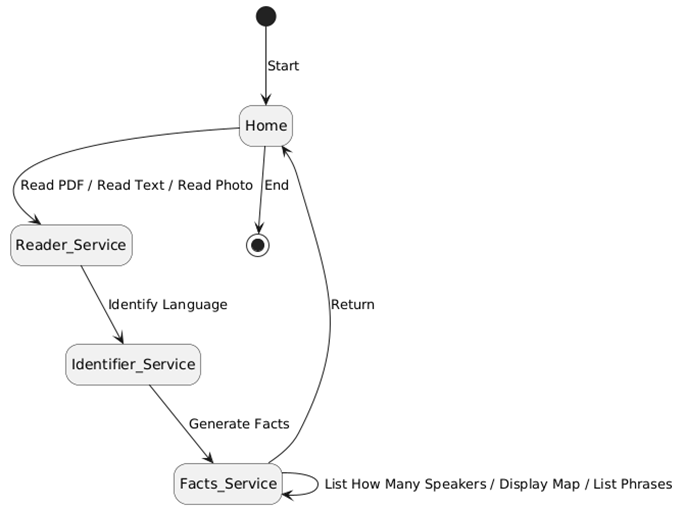
\includegraphics{Section2/State_Diagram.png}
	\caption{State Diagram}
	\label{StateDiagram}
\end{figure}
% End SubSection


\subsection{User Characteristics}
\label{sub:user_characteristics}
% Begin SubSection
\begin{itemize}
	\item \textbf{Experience}: with Application: The user may range anywhere from being a first-time user to having many experiences with the application.
	\item \textbf{Experience}: with Technology: The user has at least one month of experience using a smartphone and can perform basic actions such as taking photos, selecting a file for upload, and typing into a text box.
	\item \textbf{Education}: The user can read and write in English. They have a very basic knowledge about geography, world languages, and culture. 
	\item \textbf{Age}: The user is at least 13 years old but is likely an older teen or adult.
	\item \textbf{Physical}: Ability:  The user may be able-bodied or disabled.
	\item \textbf{Location}: The user is likely located in a culturally diverse area, whether that is due to travel or residence.
	\item \textbf{Personality}: The user is likely curious about other cultures and languages.
\end{itemize}

% End SubSection

\subsection{Constraints}
\label{sub:constraints}
% Begin SubSectionf
\begin{itemize}
	\item \textbf{Budget}: The budget is a significant constraint on the developers' options. There are costly APIs, design tools, and hosting infrastructure that can either significantly improve the quality of the product or streamline its development. Since this is a school project, the allotted budget is \textdollar 0, which leaves these products unavailable to developers. [4]
	\item \textbf{Time}: The product must be completed by the end of the term, which is in just a little over 2 months. This short timeframe means that the product will have limited features and possibly limited functionality.
	\item \textbf{Platform}: The product must be a mobile application designed for Android Operating System. This constrains the developer to make an application layout that fits the dimensions of smartphones. The functions of the application must be limited to ones that are available for the Android Operating System and mobile devices. Finally, the size of the application must fit within the phone's memory.
\end{itemize}

% End SubSection

\subsection{Assumptions and Dependencies}
\label{sub:assumptions_and_dependencies}
% Begin SubSection
\begin{itemize}
	\item List any assumptions you made in interpreting what the software being developed is aiming to achieve
	\item List any other assumptions you made that, if it fails to hold, could require you to change the requirements
	%\item List each of the factors that affect the requirements stated in the SRS
	%\item These factors are not design constraints on the software but are, rather, any changes to them that can affect the requirements in the SRS
	\begin{itemize}
		\item \textbf{Example}: An assumption may be that a specific operating system will be available on the hardware designated for the software product. If, in fact, the operating system is not available, the SRS would then have to change accordingly.
	\end{itemize}
\end{itemize}
% End SubSection

\subsection{Apportioning of Requirements}
\label{sub:apportioning_of_requirements}
% Begin SubSection
\begin{itemize}
	\item Identify requirements that may be delayed until future versions of the system
\end{itemize}
% End SubSection

% End Section


% SECTION 3
\section{Use Case Diagram}
\label{sec:use_case_diagram}
% Begin Section
\begin{itemize}
	\item Provide the use case diagram for the system being developed.
	\item You do not need to provide the textual description of any of the use cases here (these will be specified under "Highlights of Functional Requirements").
	%	\item Provide \emph{one} use case diagram for the most important Business Event.
	%	\item The text of all use cases will be specified under "Highlights of Functional Requirements"
\end{itemize}


\begin{figure}
	% \includegraphics[width=\linewidth]{Example_Use_Case.png}
	\includegraphics[width=\linewidth]{Section3/Example_Use_Case.png}
	\caption{Use Case Diagram}
	\label{UseCaseDiagram}
\end{figure}
%In this section, select the most important Business Event that your system responds to and give its use case diagram.  Only one use case diagram is needed.  Give a brief textual description of the use case without repeating what is in the scenarios of the corresponding Business Event.

%
%
%
%This section should provide a use case diagram for your application. 
%\begin{enumerate}[a)]
%	\item Each use case appearing in the diagram should be accompanied by a text description. 
%\end{enumerate}
%% End Section


% SECTION 4
\section{Highlights of Functional Requirements}
\label{sec:functional_requirements}

\noindent {\bf Main Business Events}

\begin{itemize}
	\item BE1: Identify the Language
	\item BE2: Provide Feedback to the Company
	\item BE3: Update (Add/Remove) Experts within the System
	\item BE4: Rate Experts' Results
\end{itemize}

\noindent {\bf Viewpoints}
\begin{itemize}
	\item VP1: Users
	\item VP2: Administrators
	\item VP3: Linguistic Enthusiasts
	\item VP4: Language Translator Companies
\end{itemize}


% OMITTED FOR NOW!
% \noindent {\bf Interpretation}
% \begin{itemize}
% 	\item The app 
% \end{itemize}

\begin{enumerate}[{\bf BE1:}]
	% BUSINESS EVENT# 1
	\item Identify the Language \\
		\textbf{Precondition:} User is unfamiliar with the language when browsing his/her device and decides to copy and paste said text into the app.
		\begin{enumerate}[{\bf VP1:}]
			% VIEWPOINT USER FOR BE1
			\item Users \\
				\textbf{Main Success Scenario:}
					\begin{enumerate}[{\bf 1.}]
						\item User enters the app.
						\item User taps the button to identify the language.
							\item System prompts user for input.
							\item User chooses type of input.
							\item User uploads the input onto the app (see BE2 for more details).
							\item System interprets the input.
							\item System outputs the most correct language.
					\end{enumerate}
					\textbf{Secondary Scenario:}
					\begin{enumerate}[{\bf 7.i.}]
						\item System is unable to identify the language with 80\% certainty.
						\item System asks the user for more input
					\end{enumerate} 
					\begin{enumerate}[{\bf 8.}]
						\item System is unable to identify the language with 80\% certainty
						\item System asks for user for more input
					\end{enumerate} 
			\item Admin
				\begin{enumerate}[resume]
					\item Admins gains stats
				\end{enumerate}
			\item Linguistic Enthusiasts - \textbf{N/A}
			\item Language Translator companies - \textbf{N/A}
		\end{enumerate}
	% END OF BUSINESS EVENT# 1

	

	% BUSINESS EVENT# 2
	\item Update (add/remove) the system
	\begin{enumerate}[{\bf VP1.}]
		\item Users
		\textbf{Main Success Scenario:}
		\begin{enumerate}[{\bf 1.}]
			\item User taps input button 
			\item System prompts user for input by showing different inputs and directions for each type of valid input type
			\item User selects the input option button his/her input is  related to
			\item System shows the instructions (in detail) on the type of input to upload
			\item User follows the instructions and uploads the input correctly
			\item System checks the input for any input flaws before validation
			\item System display message to user indicating the input has successfully uploaded
		\end{enumerate}
	\end{enumerate}
	% END OF BUSINESS EVENT# 2

	% BUSINESS EVENT# 3
	\item Give feedback to Languify
	\begin{enumerate}[{\bf VP1.}]
		\item Users
		\begin{enumerate}[{\bf 1.}]
			\item User enters app
			\item System displays User Interface
			\item User taps sends feedback button
			\item System prompts for user’s input
			\item User uploads experience of using app
			\item System processes and log
			
		\end{enumerate}
		\item Admin
		\begin{enumerate}[{\bf 1.}, resume]
			\item Admin checks feedback box
			\item System displaces list of feedback
			
		\end{enumerate}
		\item Linguistics Enthusiasts
		\begin{enumerate}[{\bf 4.i}]
			\item Linguistic Enthusiast points out wrong result of language identification
		\end{enumerate}
		\item Language Translator Company - \textbf{N/A}
	\end{enumerate}
	% END OF BUSINESS EVENT# 3


	% START OF BUSINESS EVENT# 4
	\item Update (Add / Remove) Experts in the system 
	\textbf{Precondition}: System is deployed and there have already existed some experts to remove or add.
	\begin{enumerate}[{\bf VP1.}]
		\item Users - \textbf{N/A}
		\item Admin
		\begin{enumerate}
			\item Admin enters APP
			\item System displays Admin Interface
			\item Admin enter Expert Managements
			\item System displays Management page
			\item Admin add/remove experts
			\item System process and display successfully process page

		\end{enumerate}
		\item Linguistics Enthusiasts - \textbf{N/A}
		\item Language Translator Company - \textbf{N/A}
	\end{enumerate}
	% END OF BUSINESS EVENT# 4


	% START OF BUSINESS EVENT #5
	\item Rate experts result 
	\begin{enumerate}[{\bf VP1.}]
		\item Users
		\begin{enumerate}[{\bf 1.}]
			\item User tapes the button of rate expert.
			\item System displays a range of one star to five star
			\item User chooses rates for each expert.
			\item System collects feedback and logs it
		\end{enumerate}
		\item Admin
		\begin{enumerate}[{\bf 6.}]
			\item System notifies Admin
			\item Admin acknowledges the feedback
		\end{enumerate}
		\item Linguistics Enthusiasts - \textbf{N/A}
		\item Language Translator Company - \textbf{N/A}
	\end{enumerate}
	% END OF BUSINESS EVENT #5
\end{enumerate}


% \begin{enumerate}[{\bf BE1.}]
% 	\item Business Event Name \#1
% 		\begin{enumerate}[{\bf VP1.}]
% 			\item Viewpoint Name \#1 \\
% 				\textcolor{red}{Insert Scenario Here}
% 			\item Viewpoint Name \#2 \\
% 				\textcolor{red}{Insert Scenario Here}
% 		\end{enumerate}
% 		{\bf Global Scenario:}\\
% 		\textcolor{red}{Insert Scenario Here}
% 	\item Business Event Name \#2
% 	\begin{enumerate}[{\bf VP1.}]
% 		\item Viewpoint Name \#1 \\
% 		\textcolor{red}{Insert Scenario Here}
% 		\item Viewpoint Name \#2 \\
% 		\textcolor{red}{Insert Scenario Here}
% 	\end{enumerate}
% 	{\bf Global Scenario:}\\
% 	\textcolor{red}{Insert Scenario Here}
% \end{enumerate}

% 	Below, we organize by Business Event.
% 	\begin{enumerate}[{BE}1.]
% 		\item Business Event name
% 		\begin{enumerate}[{VP1}.1]
% 			\item Viewpoint name \newline
% 			\noindent\fbox{%
% 				\parbox{0.5\textwidth}{%
% 					\begin{itemize}
% 						\item {\bf $S_{1}$:} Initial response of the system to the Business Event
% 						\item {\bf $E_{1}$:}  Reaction of the environment to $S_{1}$
% 						\item {\bf $S_{2}$:}  Response of the system to $E_{1}$
% 						\item {\bf $E_{2}$:}  Reaction of the environment to $S_{2}$
% 						\item[] $\cdots$
% 						\item {\bf $S_{n}$:}  Response of the system to $E_{(n-1)}$
% 						\item {\bf $E_{n}$:}  Reaction of the environment to $E_{(n-1)}$
% 						\item {\bf $S_{(n+1)}$:} Final response of the system concluding its function regarding the Business Event
% 					\end{itemize}
% 				}%
% 			}
% 			\item Viewpoint name\newline
% 			\noindent\fbox{%
% 				\parbox{0.5\textwidth}{%
% 					\begin{itemize}
% 						\item {\bf $S_{1}$:} Initial response of the system to the Business Event
% 						\item {\bf $E_{1}$:}  Reaction of the environment to $S_{1}$
% 						\item {\bf $S_{2}$:}  Response of the system to $E_{1}$
% 						\item {\bf $E_{2}$:}  Reaction of the environment to $S_{2}$
% 						\item[] $\cdots$
% 						\item {\bf $S_{k}$:}  Response of the system to $E_{(k-1)}$
% 						\item {\bf $E_{k}$:}  Reaction of the environment to $E_{(k-1)}$
% 						\item {\bf $S_{(k+1)}$:} Final response of the system concluding its function regarding the Business Event
% 					\end{itemize}
% 				}%
% 			}
% 			\item \dots
% 			\item \dots
% 			\item \dots
% 			\item[\dots]
% 		\end{enumerate}	
% 		\item[] {\bf Global Scenario of {\it Business Event Name}:} It is the scenario corresponding to the integration of all the above scenarios from the different Viewpoints of the Business Event BE1.\newline
% 		\noindent\fbox{%
% 			\parbox{0.5\textwidth}{%
% 				\begin{itemize}
% 					\item {\bf $S_{1}$:} Initial response of the system to the Business Event
% 					\item {\bf $E_{1}$:}  Reaction of the environment to $S_{1}$
% 					\item {\bf $S_{2}$:}  Response of the system to $E_{1}$
% 					\item {\bf $E_{2}$:}  Reaction of the environment to $S_{2}$
% 					\item[] $\cdots$
% 					\item {\bf $S_{m}$:}  Response of the system to $E_{(m-1)}$
% 					\item {\bf $E_{m}$:}  Reaction of the environment to $E_{(m-1)}$
% 					\item {\bf $S_{(m+1)}$:} Final response of the system concluding its function regarding the Business Event
% 				\end{itemize}
% 			}%
% 		}	
% 		%\end{enumerate}
% 		\item Business Event name
% 		\begin{enumerate}[{VP1}.1]
% 			\item Viewpoint name \newline
% 			\noindent\fbox{%
% 				\parbox{0.5\textwidth}{%
% 					\begin{itemize}
% 						\item {\bf $S_{1}$:} Initial response of the system to the Business Event
% 						\item {\bf $E_{1}$:}  Reaction of the environment to $S_{1}$
% 						\item {\bf $S_{2}$:}  Response of the system to $E_{1}$
% 						\item {\bf $E_{2}$:}  Reaction of the environment to $S_{2}$
% 						\item[] $\cdots$
% 						\item {\bf $S_{n'}$:}  Response of the system to $E_{(n'-1)}$
% 						\item {\bf $E_{n'}$:}  Reaction of the environment to $E_{(n'-1)}$
% 						\item {\bf $S_{(n'+1)}$:} Final response of the system concluding its function regarding the Business Event
% 					\end{itemize}
% 				}%
% 			}
% 			\item Viewpoint name\newline
% 			\noindent\fbox{%
% 				\parbox{0.5\textwidth}{%
% 					\begin{itemize}
% 						\item {\bf $S_{1}$:} Initial response of the system to the Business Event
% 						\item {\bf $E_{1}$:}  Reaction of the environment to $S_{1}$
% 						\item {\bf $S_{2}$:}  Response of the system to $E_{1}$
% 						\item {\bf $E_{2}$:}  Reaction of the environment to $S_{2}$
% 						\item[] $\cdots$
% 						\item {\bf $S_{k'}$:}  Response of the system to $E_{(k'-1)}$
% 						\item {\bf $E_{k'}$:}  Reaction of the environment to $E_{(k'-1)}$
% 						\item {\bf $S_{(k'+1)}$:} Final response of the system concluding its function regarding the Business Event
% 					\end{itemize}
% 				}%
% 			}
% 			\item \dots
% 			\item \dots
% 			\item \dots
% 			\item[\dots]
% 		\end{enumerate}	
% 		\item[] {\bf Global Scenario of {\it Business Event Name}:} It is the scenario corresponding to the integration of all the above scenarios from the different Viewpoints of the Business Event BE2.\newline
% 		\noindent\fbox{%
% 			\parbox{0.5\textwidth}{%
% 				\begin{itemize}
% 					\item {\bf $S_{1}$:} Initial response of the system to the Business Event
% 					\item {\bf $E_{1}$:}  Reaction of the environment to $S_{1}$
% 					\item {\bf $S_{2}$:}  Response of the system to $E_{1}$
% 					\item {\bf $E_{2}$:}  Reaction of the environment to $S_{2}$
% 					\item[] $\cdots$
% 					\item {\bf $S_{m'}$:}  Response of the system to $E_{(m'-1)}$
% 					\item {\bf $E_{m'}$:}  Reaction of the environment to $E_{(m'-1)}$
% 					\item {\bf $S_{(m'+1)}$:} Final response of the system concluding its function regarding the Business Event
% 				\end{itemize}
% 			}%
% 		}		
% 	\end{enumerate}

% End Section



% SECTION 5
\section{Non-Functional Requirements}
\label{sec:non-functional_requirements}


% Begin Section
\subsection{Look and Feel Requirements}
\label{sub:look_and_feel_requirements}
% Begin SubSection


\subsubsection{Appearance Requirements}
\label{ssub:appearance_requirements}
% Begin SubSubSection
\begin{enumerate}[{LF-A}1. ]
	\item The application shall have a simple design.
	\\ \textbf{Rationale}: A simple design helps keep users from getting overwhelmed. It will also help keep users focused on the 
	functions of the application rather than the design.
	\item The application should have text that is easily legible.
	\\ \textbf{Rationale}: Legible text contributes to ease of use and the opposite may frustrate users.
	\item The application shall have large input boxes and text boxes
	\\ \textbf{Rationale}: There is wide array of inputs the user may add. This allows for the user to make sure his/her inputs are correct and accurate
	\item The application shall haev a simple color that prevent color-blind inaccessibility
	\\ \textbf{Rationale}: Not having accessibility aspects for the application will prevent a minority of population from utilizing and testing the app  
\end{enumerate}
% End SubSubSection


\subsubsection{Style Requirements}
\label{ssub:style_requirements}
% Begin SubSubSection
\begin{enumerate}[{LF-S}1. ]
	\item The application’s components should be evenly spaced.
	\\ \textbf{Rationale}: This allows for navigation to quick and easy. The user is less prone to mistakes when he/she applies gestures for navigation
\end{enumerate}
% End SubSubSection

% End SubSection


\subsection{Usability and Humanity Requirements}
\label{sub:usability_and_humanity_requirements}
% Begin SubSection

\subsubsection{Ease of Use Requirements}
\label{ssub:ease_of_use_requirements}
% Begin SubSubSection
\begin{enumerate}[{UH-EOU}1. ]
	\item The system must allow users to report bugs within the application.
	\\ \textbf{Rationale}: With these reports about bugs within the application, the developers can then investigate and fix the bug to further improve the application.
	\item The system must allow users to send feedback about the application within the application.
	\\ \textbf{Rationale}: With feedback received from the users about the application, the developers can then utilize that feedback and further improve the application.
	\item The system must only prompt the user when decisions and confirmations are required.
	\\ \textbf{Rationale}: If the user is constantly getting prompted unnecessarily, the user will become more annoyed with the application and will have a higher chance in leaving the application.
\end{enumerate}
% End SubSubSection


\subsubsection{Personalization and Internationalization Requirements}
\label{ssub:personalization_and_internationalization_requirements}
% Begin SubSubSection
\begin{enumerate}[{UH-PI}1. ]
	\item The system shall allow the user to select the preferred language used within the application.
	\\ \textbf{Rationale}: Users would then be able to navigate and have a better overall experience with the application when they are able to understand it more easily. Thus, this would then encourage the user to continue using the application in the future.
	\item The system shall allow the user to customize what phrases of the identified language are given to them.
	\\ \textbf{Rationale}: Users would then find more enjoyment while using the application when they can tailor what they want to learn how to say in the language being identified.
\end{enumerate}
% End SubSubSection


\subsubsection{Learning Requirements}
\label{ssub:learning_requirements}
% Begin SubSubSection
\begin{enumerate}[{UH-L}1. ]
	\item The user should be able to figure out how to use the application for the first time without any instruction within 5 minutes.
	\\ \textbf{Rationale}: If the user must spend more than 5 minutes trying to figure out the application or must read a long instruction manual to figure out how to use the application, the user will then become frustrated and abandon the application. This would then discourage the user for ever using the application in the future when they would be frustrated every time they try to use the application.	
\end{enumerate}
% End SubSubSection

\subsubsection{Understandability and Politeness Requirements}
\label{ssub:understandability_and_politeness_requirements}
% Begin SubSubSection
\begin{enumerate}[{UH-UP}1. ]
	\item The user should be able to use the application smoothly and get a result within 5 minutes of operation.
	\\ \textbf{Rationale}: If the application is self-intuitive, easy to use, and fast, it would encourage the user to keep using the application and continue using it within the future due to these benefits.
	\item The system shall use proper manners and etiquette whenever the user is prompted to decide or input something.
	\\ \textbf{Rationale}: If the user feels as if they are being offended or being rude towards, the user would then abandon the application and spread a bad reputation towards the application to other users.
\end{enumerate}
% End SubSubSection


\subsubsection{Accessibility Requirements}
\label{ssub:accessibility_requirements}
% Begin SubSubSection
\begin{enumerate}[{UH-A}1. ]
	\item The system should be able to switch colour settings between a normal colour palette, to other colour palettes such as the Protan and Deutan colour palettes [], to accommodate people with colour blindness.
	\\ \textbf{Rationale}: Users who are colourblind will then be able to differentiate between different parts of the application but also be able to use the functionality of the application with more ease.
	
\end{enumerate}
% End SubSubSection

% End SubSection

\subsection{Performance Requirements}
\label{sub:performance_requirements}
% Begin SubSection

\subsubsection{Speed and Latency Requirements}
\label{ssub:speed_and_latency_requirements}
% Begin SubSubSection
\begin{enumerate}[{PR-SL}1. ]
	\item The response time of all the APIs used in app should be less than 1second.
	\\ \textbf{Rationale}: APIs have response time between 0.1s and 1s will improve user experience and increase competitive. 	Response time out of this range will mean that users will face minor delays (1s to 2s) and might suffer and choose 	other application instead.
	\item The response time of Identification must limit in 5 second.
	\\ \textbf{Rationale}: The response time of Identification is not critical as response time of API, since experts need to analyze the 	input from user. However, the waiting time for result must not be that long in order to affect user experience of app.
	\item The app startup time should be less than 2 seconds.
	\\ \textbf{Rationale}: Too long time for startup will affect user experience and user would like to switch to another faster startup time app.
\end{enumerate}
% End SubSubSection


\subsubsection{Safety-Critical Requirements}
\label{ssub:safety_critical_requirements}
% Begin SubSubSection
% \begin{enumerate}[{PR-SC}1. ]
	\textbf{N/A}
% \end{enumerate}
% End SubSubSection

\subsubsection{Precision or Accuracy Requirements}
\label{ssub:precision_or_accuracy_requirements}
% Begin SubSubSection
\begin{enumerate}[{PR-PA}1. ]
	\item The app must show the most precise result of identification.
	\\ \textbf{Rationale}: The accuracy of result from system are corresponding to the quality of input. The system sometime make error when lack of information.
	\item The average of all ratings made for a user in the app must be accurate up to one decimal place
	\\ \textbf{Rationale}: In order to keep the UI simple for rating, our app users only one decimal place for ratings and this is followed by other apps in the industry. 
\end{enumerate}
% End SubSubSection

\subsubsection{Reliability and Availability Requirements}
\label{ssub:reliability_and_availability_requirements}
% Begin SubSubSection
\begin{enumerate}[{PR-RA}1. ]
	\item The system must have an availability of 99.9\% except for maintenance and Internet networks go down
	\\ \textbf{Rationale}: The longer availability will make the app more competitive; it should have an availability of 99.9\% (three nines) as most of the application in the industry aim to have that percentage [1]. That means app will have downtime of 8.76 hours per year for maintenance and other exception. This allows time for updating new expert in system and solve unexpected crash of system.
	\item The system must create backups of all the app data
	\\ \textbf{Rationale}: In case some unexpected things happened, system could lose all the feedback and information from user, having a backup of that data will ensure us to recover our lost data.
\end{enumerate}
% End SubSubSection


\subsubsection{Robustness or Fault-Tolerance Requirements}
\label{ssub:robustness_or_fault_tolerance_requirements}
% Begin SubSubSection
\begin{enumerate}[{PR-RFT}1. ]
	\item The user must be able to enter input that system could parse (ex pdf, txt, text) even when app is not connected to the internet. However, the result provided by the system will not return to the user until the internet connection is restored.
	\\ \textbf{Rationale}: Even user cannot access the Internet, they should still be able to enter they input as they would not have to enter them again once the internet connection is restored.
	\item The system must be able to handle exceptional input made by the user
	\\ \textbf{Rationale}: If the input is exceptional, then the app should not crash and instead fail gracefully
\end{enumerate}
% End SubSubSection

\subsubsection{Capacity Requirements}
\label{ssub:capacity_requirements}
% Begin SubSubSection
\begin{enumerate}[{PR-C}1. ]
	\item The system must be able to handle 10 simultaneous request
	\\ \textbf{Rationale}: Considering the scope of the project, this requirement can be verified without taking much time	
\end{enumerate}
% End SubSubSection

\subsubsection{Scalability or Extensibility Requirements}
\label{ssub:scalability_or_extensibility_requirements}
% Begin SubSubSection
\begin{enumerate}[{PR-SE}1. ]
	\item The code for the system must open to addition and close to modification.
	\\ \textbf{Rationale}: By applying this principle ensure not only stability and consistency (close to modification) and maximize 	the scalability and extensibility as well.
\end{enumerate}
% End SubSubSection

\subsubsection{Longevity Requirements}
\label{ssub:longevity_requirements}
% Begin SubSubSection
\textbf{N/A}
% \begin{enumerate}[{PR-L}1. ]
% 	\item 
% \end{enumerate}
% End SubSubSection

% End SubSection

\subsection{Operational and Environmental Requirements}
\label{sub:operational_and_environmental_requirements}
% Begin SubSection

\subsubsection{Expected Physical Environment}
\label{ssub:expected_physical_environment}
% Begin SubSubSection
\begin{enumerate}[{OE-EPE}1. ]
	\item The system must be compatible with ARM architecture paired with both android and iOS operating systems.
	\\ \textbf{Rationale}: Each expert must interact with the central database to reference their respective data stores, and obtain necessary language information. A max latency of 1 second ensures fast communication between both parties so that the language is deduced in a sensible time. 
\end{enumerate}
% End SubSubSection

\subsubsection{Requirements for Interfacing with Adjacent Systems}
\label{ssub:requirements_for_interfacing_with_adjacent_systems}
% Begin SubSubSection
\begin{enumerate}[{OE-IA}1.]
	\item The system must perform two-way communication with a cloud database in at most 1 second.
	\textbf{Rationale}: Each expert must interact with the central database to reference their respective data stores, and obtain necessary language information. A max latency of 1 second ensures fast communication between both parties so that the language is deduced in a sensible time.   
	\item The system must be able to send JPEG, HEIC, and PNG images of up to 100MB to a computer vision API, and receive information without disruption.
	\\ \textbf{Rationale}: Phones that use iOS (iPhone) store images in HEIC or JPEG by default. Phones that use Android operating systems most commonly store them in JPEG and PNG [3]. Image sizes of up to 100MB ensure high quality pictures are transferable between the system and API.
	\item The system must be able to dynamically send country names and receive a corresponding photo from an image generator API.
	\\ \textbf{Rationale}: The innovative feature requires that images must be able to dynamically produce a map highlighting countries with prominent speakers for certain languages.
\end{enumerate}
% End SubSubSection

\subsubsection{Productization Requirements}
\label{ssub:productization_requirements}
% Begin SubSubSection
\textbf{N/A}
% \begin{enumerate}[{OE-P}1. ]
% 	\item 
% \end{enumerate}
% End SubSubSection

\subsubsection{Release Requirements}
\label{ssub:release_requirements}
% Begin SubSubSection
\begin{enumerate}[{OE-R}1. ]
	\item The system must be compatible with Android 12.0, iOS 18.0, or above.
	\\ \textbf{Rationale}: Both iOS and android operating systems are used by the app, and these are their last versions that receive active maintenance and security support [4][5]. 
	\item The deployed system must have a maximum downtime or 1 hour per 2 weeks.
	\\ \textbf{Rationale}: The product must be available to use for as long as possible, and 1 hour per week leaves sufficient time to deploy maintenance updates and bug fixing.
	\item The system must only be accessible for users with a network connection of at least 2 Mb/s.
	\\ \textbf{Rationale}: To guarantee all API and database communication functions as expected, a stable network connection is necessary. These calls apply a load comparable to those made when browsing the web, where a speed of 2-5 Mb/s is satisfactory [6].
\end{enumerate}
% End SubSubSection

\textbf{NOTE: FIX THE REFERENCE NUMBERS ON THESE}

% End SubSection

\subsection{Maintainability and Support Requirements}
\label{sub:maintainability_and_support_requirements}
% Begin SubSection

\subsubsection{Maintenance Requirements}
\label{ssub:maintenance_requirements}
% Begin SubSubSection
\begin{enumerate}[{MS-M}1. ]
	\item The system must have minimum monthly software updates to patch bugs in the software  
	\\ \textbf{Rationale}: To ensure system 	run smoothly and that bugs get patched and fixed regularly. This will help to maintain 	good app quality throughout its use.
	\item The system must have minimum three times per year to expand and update languages libraries. 
	\\ \textbf{Rationale}: To ensure the new created slangs and words are added into library to help identify language.
\end{enumerate}
% End SubSubSection

\subsubsection{Supportability Requirements}
\label{ssub:supportability_requirements}
% Begin SubSubSection
\begin{enumerate}[{MS-S}1. ]
	\item The system must support different operate system of phone such as IOS, Android are able to use the app. 
	\\ \textbf{Rationale}: To ensure that the large variety of phone user could get supported by the app. 
\end{enumerate}
% End SubSubSection

\subsubsection{Adaptability Requirements}
\label{ssub:adaptability_requirements}
% Begin SubSubSection
\begin{enumerate}[{MS-A}1. ]
	\item The system shall be able to run on the most current Android release on Android devices 
	\\ \textbf{Rationale}: To ensure that the app is compatible with older and new android devices
\end{enumerate}
% End SubSubSection

% End SubSection

\subsection{Security Requirements}
\label{sub:security_requirements}
% Begin SubSection

\subsubsection{Access Requirements}
\label{ssub:access_requirements}
% Begin SubSubSection
\begin{enumerate}[{SR-AC}1. ]
	\item The app must ask the user for file storage, paste board and photos of the device to acquire the input 
	\\ \textbf{Rationale}: The system must ask the permission of accessing format that stores text in order to identify language. 
\end{enumerate}
% End SubSubSection

\subsubsection{Integrity Requirements}
\label{ssub:integrity_requirements}
% Begin SubSubSection
\textbf{N/A}
% \begin{enumerate}[{SR-INT}1. ]
% 	\item 
% 	\textbf{Rationale}:
% \end{enumerate}
% End SubSubSection

\subsubsection{Privacy Requirements}
\label{ssub:privacy_requirements}
% Begin SubSubSection
\begin{enumerate}[{SR-P}1. ]
	\item The app must ensure the confidentiality of user input. 
	\\ \textbf{Rationale}: Input from user to identify the language should not leak to anyone 
\end{enumerate}
% End SubSubSection

\subsubsection{Audit Requirements}
\label{ssub:audit_requirements}
% Begin SubSubSection
\textbf{N/A}
% \begin{enumerate}[{SR-AU}1. ]
% 	\item 
% 	\textbf{Rationale}:
% \end{enumerate}
% End SubSubSection

\subsubsection{Immunity Requirements}
\label{ssub:immunity_requirements}
% Begin SubSubSection
\begin{enumerate}[{SR-IM}1. ]
	\item The system must not accept unexpected input
	\\ \textbf{Rationale}: This is to prevent attacks like SQL Injection.
\end{enumerate}
% End SubSubSection

% End SubSection

\subsection{Cultural and Political Requirements}
\label{sub:cultural_and_political_requirements}
% Begin SubSection

\subsubsection{Cultural Requirements}
\label{ssub:cultural_requirements}
% Begin SubSubSection
\begin{enumerate}[{CP-C}1. ]
	\item The system must not contain any words that can be considered offensive ( to any religion, ethnicity, disability, sexual orientation, groups) where the app is available, utilizing a list of unacceptable words for reference.
	\\ \textbf{Rationale}: To ensure people feel safe when using the app.  Any words well known to be offensive must purposely be 	excluded from any designs or usage in the system. 
\end{enumerate}
% End SubSubSection

\subsubsection{Political Requirements}
\label{ssub:political_requirements}
% Begin SubSubSection
\textbf{N/A}
% \begin{enumerate}[{CP-P}1. ]
% 	\item 
% 	\textbf{Rationale}:
% \end{enumerate}
% End SubSubSection

% End SubSection

\subsection{Legal Requirements}
\label{sub:legal_requirements}
% Begin SubSection

\subsubsection{Compliance Requirements}
\label{ssub:compliance_requirements}
% Begin SubSubSection
\begin{enumerate}[{LR-COMP}1. ]
	\item The system must convey that all images passed into the system are to be analyzed by computer vision algorithms prior to any collection.
	\\ \textbf{Rationale}: Based on PIPEDA Principle 2, the purpose of collected data must be specified by the organization before or during the time of collection [7]. All apps launched in Canada must comply with PIPEDA regulations.
	\item All images processed with computer vision algorithms must ensure that only text is extracted and analyzed.
	\\ \textbf{Rationale}: Based on PIPEDA Principle 4, only data that is necessary for the system is collected [7]. So, any other visible artifacts including, but not limited to addresses, signatures and people cannot be analyzed.
	\item Collected images are discarded upon analysis of the text. The text is also discarded when the user prompts to close the window.
	\\ \textbf{Rationale}: Based on ISO 27001, data must be encrypted when it is being transmitted between parties to prevent leakage of any IP addresses and other personal data [8].
\end{enumerate}
% End SubSubSection

\subsubsection{Standards Requirements}
\label{ssub:standards_requirements}
% Begin SubSubSection
\begin{enumerate}[{LR-STD}1. ]
	\item The system must ensure that text is resizable, and that the interface’s colour contrast satisfies the Web Content Accessibility Guidelines.
	\\ \textbf{Rationale}: This is a key standard outlined in the AODA, which applies to Languify as it is developed and released in Ontario [9].
	\item The system shall offer a virtual keyboard for each supported script, which is controllable with the physical keyboard’s arrow keys. Each screen must be fully navigable with the physical keyboard as well.
	\\ \textbf{Rationale}: As per the AODA, systems must be navigable without a mouse to be considered operable [9]. This also ensures it is usable under any conditions.
	\item The system shall provide clearly labelled buttons, input modules, and instructions for every functionality.
	\\ \textbf{Rationale}: As per the AODA, systems must be understandable, with unambiguous wording and input assistance to make them as easy to use as possible [9].
	\item The system must be compatible with screen readers and provide alternative text when needed.
	\\ \textbf{Rationale}: As per the AODA, it is crucial to follow proper coding standards and semantics so that they are accessible to as many audiences as possible [9].
\end{enumerate}
% End SubSubSection

% End SubSection

% End Section

% SECTION 6
\section{Innovative Features}
\label{sec:innovative_features}

% BEGIN SECTION

To supplement the language detector application’s base functionality, the system introduces two innovative features: photographic text recognition and language datasheets.\\

At the base level, users type out the text they wish to inquire about. However, there is a flaw with this method – if the user does not recognize the language, it is highly unlikely that they have a keyboard that supports its alphabet. Even if they do, they lack the knowledge to write out the characters quickly. The lack of intuition behind this input method incentivizes users to use competitor apps instead, taking away from the company’s revenue. So to rectify this concern, instead of requesting a whole typed out string from the user, the photo recognizer simply takes one picture as input, and internally extracts the writing. With the snap of one picture, the system autonomously identifies the correct language, making it the most convenient option available. This way, it sustains all of its users, leading to increased usage and revenue.\\

To further enhance the user experience, the system displays informational datasheets corresponding to the languages when they are scanned. Queries are rewarded with a comprehensive set of fun facts about the language’s scripts, history, speakers, and with prominent regions that speak the language pinpointed on a map.\\

Overall, the superior ease of use and informativity when identifying the language separates this app from alternatives. These benefits drive more users to the app, and in turn, increases revenue for the company.\\  

Some other features that are considered in future updates include: 
\begin{itemize}
    \item Translator Service
    \item Audio Interpreter
    \item Profile Feature to track app usage and recent scans 
    \item Language Quizzes
    \begin{itemize}
        \item One vs One with Friends 
        \item Global Tournaments
    \end{itemize}
    \item Geo-Assigning Languages based on High Scan Locations 
    \begin{itemize}
        \item For example, if a French speaking student is planning to attend McMaster University and sees a lot of students scan French text east of the university, whereas the west is more English dominated, they might choose to move into the eastern part as it's likely that more people of the same culture live there. 
    \end{itemize}
    \item Machine Learning Model Expert
\end{itemize}

% END SECTION


% DIVISION OF LABOR
\appendix
\section{Division of Labour}
\label{sec:division_of_labour}
% Begin Section

\textbf{Andy Huynh}
\begin{itemize}
    \item Worked on Section 4 Business Events with Ke Ma
    \item Set up and translated all the text into the LaTeX file
    \item Worked on Sections 5.5, 5.6, and 5.7 with Ke Ma
\end{itemize}
\begin{figure}[H]
	\centering
	
\includegraphics[width=0.2\textwidth]{Signatures/a.png}  
\end{figure}

\textbf{Cheukman Zhou}
\begin{itemize}
    \item Worked on Section 1.2
    \item Worked on Section 3.1
    \item Helped with formatting and editing of the document on LaTeX
\end{itemize}
\begin{figure}[H]
	\centering
	
\includegraphics[width=0.2\textwidth]{Signatures/c.png}
\end{figure}

\textbf{Ke Ma}
\begin{itemize}
    \item Worked on Section 4 with Andy Huynh
    \item Worked on Sections 5.5, 5.6, and 5.7 with Andy Huynh
\end{itemize}
\begin{figure}[H]
	\centering
	
\includegraphics[width=0.2\textwidth]{Signatures/k.png}
\end{figure}

\textbf{Sarah Dorfman}
\begin{itemize}
    \item Worked on Section 2 alongside Cheukman Zhou
    \item Worked on Section 5.1
\end{itemize}
\begin{figure}[H]
	\centering
	
\includegraphics[width=0.2\textwidth]{Signatures/s.png}
\end{figure}

\textbf{Gurmanjot Minhas}
\begin{itemize}
    \item Worked on Section 3
    \item Worked on Sections 5.4 and 5.8
    \item Completed Section 6: Innovative Ideas
\end{itemize}
\begin{figure}[H]
	\centering
	
\includegraphics[width=0.2\textwidth]{Signatures/g.png}
\end{figure}

% End Section


\end{document}
%------------------------------------------------------------------------------